\documentclass[tikz]{standalone}
\usepackage{ctex}
\usepackage{tikz}
\usepackage{pgfplots}
\pgfplotsset{compat=1.18}   % 使用较新版本语法
\usetikzlibrary{positioning, arrows.meta, intersections, calc, fit, backgrounds}
\usepgfplotslibrary{fillbetween}  % 用于填充区域

\begin{document}
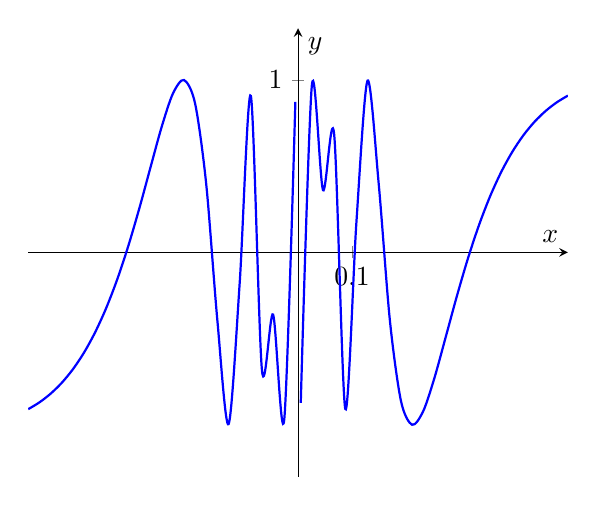
\begin{tikzpicture}
    \begin{axis}[
            % width=0.45\textwidth,
            axis lines = middle,
            xlabel = $x$, ylabel = $y$,
            xmin = -0.5, xmax = 0.5,
            ymin = -1.3, ymax = 1.3,   % 缩小 y 范围，突出变化
            xtick = {0,0.1},
            xticklabels = {0,0.1},
            ytick = {1},
            yticklabels = {1},
            % axis equal = true,       % 去掉或注释掉
            clip = true,
            every axis plot post/.append style={thick}
        ]
        \addplot[blue, domain=-0.5:-0.005, smooth] {sin(deg(1/x))};
        \addplot[blue, domain=0.005:0.5, smooth] {sin(deg(1/x))};
    \end{axis}
\end{tikzpicture}
\end{document}